\documentclass[12pt,a4paper]{article}
\usepackage{fontspec}
\IfFontExistsTF{Times New Roman}{\setmainfont{Times New Roman}}{\setmainfont{DejaVu Serif}[ItalicFont={DejaVu Serif},ItalicFeatures={FakeSlant=0.15},BoldItalicFont={DejaVu Serif Bold},BoldItalicFeatures={FakeSlant=0.15}]}
\setsansfont{DejaVu Sans}
\setmonofont[Scale=0.85]{DejaVu Sans Mono}
\usepackage[left=3cm,right=2cm,top=2cm,bottom=2cm]{geometry}
\usepackage{graphicx,booktabs,tabularx,array,longtable,float}
\usepackage{enumitem,setspace,titlesec,fancyhdr,xcolor}
\usepackage{listings,xurl}
\usepackage[hidelinks,unicode]{hyperref}
\usepackage{caption,tocloft}
\setlength{\cftsecnumwidth}{2.2em}
\setlength{\cftsubsecnumwidth}{2.7em}
\setstretch{1.15}
\setlength{\parindent}{1.1cm}
\setlength{\parskip}{3pt}
\setlength{\emergencystretch}{2em}
\setlist{nosep,leftmargin=1.6em,topsep=4pt}
\renewcommand{\contentsname}{Гарчиг}
\renewcommand{\figurename}{Зураг}
\renewcommand{\tablename}{Хүснэгт}
\captionsetup{font=small,labelfont=bf}
\titleformat{\section}{\large\bfseries}{\thesection.}{0.6em}{}
\titleformat{\subsection}{\normalsize\bfseries}{\thesubsection.}{0.6em}{}
\titlespacing*{\section}{0pt}{12pt}{7pt}
\titlespacing*{\subsection}{0pt}{8pt}{5pt}
\pagestyle{fancy}
\fancyhf{}
\fancyhead[L]{\small F.CSM302 Үйлдлийн систем}
\fancyhead[R]{\small Бие даалт №1}
\fancyfoot[C]{\thepage}
\setlength{\headheight}{16pt}
\renewcommand{\headrulewidth}{0.3pt}
\newcolumntype{Y}{>{\raggedright\arraybackslash}X}
\newcolumntype{P}[1]{>{\raggedright\arraybackslash}p{#1}}
\newcommand{\code}[1]{\texttt{#1}}
\newcommand{\docname}{Судалгаа, хэрэгжилт, туршилтын тайлан}
\lstset{basicstyle=\ttfamily\footnotesize,breaklines=true,columns=fullflexible,keepspaces=true,
 frame=single,rulecolor=\color{black!25},backgroundcolor=\color{black!3},showstringspaces=false,
 xleftmargin=4pt,xrightmargin=4pt,aboveskip=7pt,belowskip=7pt}
\hypersetup{pdfauthor={А.Тэмүүлэн B242270063},pdftitle={Linux Kernel Module for Listing Tasks}}

\begin{document}
% User-provided MUST title-page layout, adapted for F.CSM302.
\begin{titlepage}
\begin{center}
{\large Шинжлэх Ухаан Технологийн Их Сургууль\par}
{Мэдээлэл, Холбооны Технологийн Сургууль\par}
\vspace{0.6cm}

\includegraphics[width=2.05cm]{figures/MUST_logo.png}\par
\vspace{0.8cm}
{\large F.CSM302\quad Үйлдлийн систем\par}
\vspace{1.25cm}
{\Large\bfseries Linux цөмийн модулиар процессын\par
жагсаалт ба холбоосыг дүрслэх\par}
\vspace{0.35cm}
{\normalsize Linux Kernel Module for Listing Tasks\par}
\vspace{0.65cm}
{\Large Бие даалт №1\par}
\vspace{0.25cm}
{\normalsize\docname\par}
\vspace{1.0cm}
\begin{minipage}{0.97\textwidth}
\setstretch{1.15}
\begin{tabularx}{\linewidth}{@{}P{4.0cm}Y@{}}
Шалгасан багш: & Г.Ганбат \\[0.2cm]
Багийн дугаар: & IV-2-3 \\[0.3cm]
Гүйцэтгэсэн оюутнууд: & А.Тэмүүлэн /B242270063/ \\[0.15cm]
& Ч.Балгандамба /B232270142/ \\[0.15cm]
& Д.Азмаа /B241940101/ \\[0.15cm]
& Н.Билэгт-Очир /B231910009/ \\[0.15cm]
& Т.Түвшинтөр /B190910820/ \\[0.15cm]
& Б.Өсөхбаяр /B210930901/ \\
\end{tabularx}
\end{minipage}
\vfill
{\large Улаанбаатар хот\par}
{\large 2026 он\par}
\end{center}
\end{titlepage}

\pagenumbering{roman}
\tableofcontents
\clearpage
\pagenumbering{arabic}

\section*{Хураангуй}
\addcontentsline{toc}{section}{Хураангуй}
Linux системийн процесс, thread-ийн мэдээллийг kernel module-оор уншиж, холбоосыг графаар харуулах TaskGraph програм хэрэгжүүлэв. Модуль нь PID, төлөв, нэрийг LINEAR болон DFS дарааллаар хэвлэж, \code{/proc/taskgraph} файлаар шинэ хэмжилт өгнө. UI-аас дэд мод сонгох, thread шүүх, дарааллаар үзэх, мэдээлэл хадгалах боломжтой. Python-ийн 23, бодит Linux kernel-ийн 12 шалгалт нийт 35/35 тэнцсэн.

\section{Удиртгал}
Зорилго нь Linux-ийн процессын бүтэц, эцэг-хүүхэд холбоо болон DFS аргыг бодит өгөгдөл дээр судлах юм. Процесс үүсэх, зогсох, дуусах өөрчлөлтийг граф, хүснэгтээр ажиглана. Хэрэгжилт нь C kernel module, Python parser, Tkinter UI гэсэн гурван хэсэгтэй.

\section{Сурах бичгийн шаардлага}
\textit{Operating System Concepts} сурах бичгийн 3-р бүлгийн Programming Project 3 нь task-уудыг шугаман болон гүний хайлтаар жагсаахыг шаарддаг \cite{osc}.
\begin{table}[H]
\centering\small
\caption{Үндсэн шаардлага ба хэрэгжилт}
\begin{tabularx}{\textwidth}{@{}P{3.25cm}Y@{}}\toprule
Шаардлага & Хэрэгжилт \\\midrule
Шугаман жагсаалт & \code{for\_each\_process()} ашиглаж process leader бүрийн PID, state, comm-ийг kernel log-д хэвлэнэ. \\
DFS жагсаалт & \code{init\_task}-аас эхэлсэн модыг kernel дотор стекээр туулж, дараалал ба гүнийг гаргана. \\
Зөв ажиллагааг шалгах & Process жагсаалтыг \code{ps -el}, thread-үүдийг \code{ps -eLf}-тэй харьцуулж болно. \\
Task graph UI & Parent-child болон process-thread холбоосыг дүрсэлж, дахин уншихад шинэчилнэ. \\
Өөрчилж турших & Root PID, thread шүүлт, харагдах тоо, шинэчлэх хугацааг өөрчилнө. Буруу оролтыг мэдээлнэ. \\\bottomrule
\end{tabularx}
\end{table}
Номын \code{children/sibling} холбоосыг шууд рекурсээр дагахын оронд хамгаалалттай хуулсан parent ID-аас мод байгуулсан. Ингэснээр өөрчлөгдөж буй kernel жагсаалтыг түгжээгүй дагахгүй, kernel stack дээр рекурс ашиглахгүй.

\clearpage
\section{Онолын үндэс}
Linux-ийн \code{task\_struct} нь task-ийн PID, төлөв, нэр болон холбоосыг агуулна. Нэг процесс олон thread-тэй байж болно.
\begin{itemize}
\item \textbf{PID}: task-ийн дугаар; \textbf{TGID}: thread group-ийн дугаар. Process leader-ийн PID ба TGID ижил.
\item \textbf{PPID}: эцэг процессын дугаар. Графт process-ийг PPID-тай, нэмэлт thread-ийг өөрийн TGID-тай холбоно.
\item \textbf{LINEAR}: process жагсаалтыг дарааллаар унших арга.
\item \textbf{DFS}: эхлээд эцэг зангилаа, дараа нь хүүхдийн дэд модыг бүрэн туулна.
\end{itemize}
Төлөвийн тэмдэг: R --- ажиллаж байгаа эсвэл бэлэн; S --- унтаж байгаа; I --- idle kernel thread; D --- uninterruptible sleep; T/t --- зогсоосон; Z/X --- zombie/dead.


\section{Системийн зохиомж}
Өгөгдөл \code{task\_struct} $\rightarrow$ kernel snapshot $\rightarrow$ \code{/proc/taskgraph} $\rightarrow$ Python parser $\rightarrow$ граф, хүснэгт гэсэн урсгалаар дамжина.
\begin{table}[H]
\centering\small
\caption{Компонентуудын үүрэг}
\begin{tabularx}{\textwidth}{@{}P{3.4cm}Y@{}}\toprule
Компонент & Үүрэг \\\midrule
\code{taskgraph.c} & Task-уудын мэдээллийг хуулж, parent индекс, DFS дараалал тооцно. \\
\code{model.py} & TSV өгөгдлийг шалгаж, дэд мод болон thread шүүлт хийнэ. \\
\code{gui.py}, \code{cli.py} & Нэг өгөгдлийг график болон командын мөрөөр үзүүлнэ. \\
\code{workload.py} & Өөр өөр гүн, салаалалттай туршилтын процессын мод үүсгэнэ. \\\bottomrule
\end{tabularx}
\end{table}
Snapshot бүр \code{pid, ppid, tgid, parent, state, kind, linear, dfs, depth, orphan, comm} баганатай. \code{count}, \code{cap}, \code{truncated} нь хэмжилт бүтэн эсэхийг мэдээлнэ.

\section{Хэрэгжилт}
\code{tg\_capture()} нь санах ойг урьдчилан хуваарилж, RCU хамгаалалттай үед task-ийн утгуудыг хуулна \cite{rcu}. Lock-оос гарсны дараа parent ID-аар мод байгуулж, \code{tg\_tree()} функцээр DFS гүйцэтгэнэ. Модулийг ачаалахад LINEAR ба DFS жагсаалт kernel log-д гарна.
\code{seq\_file} нь нэг нээлттэй файлаас хэсэгчлэн уншихад ижил snapshot ашиглана \cite{seq}. Дахин нээх бүр шинэ өгөгдөл авна. \code{max\_tasks} нь 16--16384, анхны утга 4096. Хязгаар хүрвэл \code{truncated=1} гэж мэдээлнэ. Parser нь формат, PID давхардал, дараалал, төлөв болон оролтын хэмжээг шалгана.

\clearpage
\section{Туршилт ба UI дүрслэл}
Зүүн хэсэгт task graph, баруун хэсэгт хүснэгт харагдана. Тасралтгүй сум нь process parent-child холбоо, тасархай сум нь thread group-ийн гишүүнчлэл юм. Зангилааг сонгоход доод мөрөнд дэлгэрэнгүй гарна.
\begin{table}[H]
\centering\small
\caption{Өөрчилж турших удирдлагууд}
\begin{tabularx}{\textwidth}{@{}P{3.5cm}Y@{}}\toprule
Удирдлага & Үйлдэл \\\midrule
DFS / LINEAR & Task үзүүлэх дарааллыг солино. \\
Root PID / Threads & Дэд мод сонгож, нэмэлт thread-үүдийг харуулна эсвэл нууна. \\
Зангилааны хязгаар & 1--2000 хүртэл task харуулна; бүтэн snapshot-ийг өөрчлөхгүй. \\
Шинэчлэх / Авто шинэчлэлт & Эх үүсвэрийг дахин уншина. Интервал 500--10000 ms. \\
Өмнөх / Дараах / Тоглуулах & Нэг snapshot дотор traversal-ийг алхмаар харуулна. \\
Файл нээх / Хадгалах / Reset & Snapshot импортлох, экспортлох, view тохиргоо сэргээх. \\\bottomrule
\end{tabularx}
\end{table}
\textbf{Kernel горим} нь бодит модулиас өгөгдөл авна. \textbf{File горим} нь хадгалсан хэмжилтийг харуулна. \textbf{Fixture горим} нь алгоритм шалгах жишээ өгөгдөлтэй. Эх үүсвэрийг дэлгэцэд ялгаж тэмдэглэсэн. File горимын автомат шинэчлэлт нь ижил файлыг дахин уншина.

\section{Туршилтын арга}
\begin{table}[H]
\centering\small
\caption{Туршсан орчин}
\begin{tabularx}{\textwidth}{@{}P{3.2cm}Y@{}}\toprule
Хэсэг & Орчин \\\midrule
Build & Ubuntu 24.04, GCC 13.3.0, Linux 6.8.0-31 headers. \\
Kernel ажиллагаа & QEMU 8.2.2 TCG, 2 vCPU, 512 MiB RAM, Linux 6.8.0-31-generic, initramfs. \\
UI, автомат тест & Python 3.12, Tk 8.6, unittest, Xvfb. \\\bottomrule
\end{tabularx}
\end{table}
Python тестээр оролт шалгах, LINEAR/DFS, дэд мод, thread шүүлт, импорт/экспорт, буруу оролт болон 5000 гүн модыг шалгав. Kernel тестээр модулийг ачаалж, процесс ба thread үүсгэн \code{before}, \code{created}, \code{stopped}, \code{after}, \code{capped} үеийн snapshot авсан.
C workload нь 5 process, нэмэлт 2 thread буюу 7 task үүсгэнэ. Root-д SIGSTOP өгөхөд T төлөв болох, дуусгахад бүх хүүхэд цэвэрлэгдэхийг шалгасан. Үр дүнг \code{docs/evidence/} дотор log, JSON, TSV хэлбэрээр хадгалсан.

\clearpage
\section{Үр дүн}
Python-ийн \textbf{23/23 тест}, kernel-ийн \textbf{12/12 шалгалт} тэнцэв. Модуль амжилттай хөрвөж, Linux 6.8.0-31 дээр ачаалагдсан.
\begin{table}[H]
\centering\small
\caption{Бодит kernel дээрх шалгалтын үр дүн}
\begin{tabularx}{\textwidth}{@{}P{0.8cm}YP{2.0cm}@{}}\toprule
Код & Ажигласан үр дүн & Төлөв \\\midrule
K1 & Модуль ачаалагдав; \code{insmod} exit=0. & Тэнцсэн \\
K2 & Kernel эх үүсвэртэй 66 task; PID 0 багтсан. & Тэнцсэн \\
K3 & LINEAR болон DFS log хоёулаа хэвлэгдсэн. & Тэнцсэн \\
K4 & 73 task-ийн DFS rank давхцаагүй; parent нь child-ээс өмнө. & Тэнцсэн \\
K5 & Root PID 90-ийн дэд мод 7 task-тай. & Тэнцсэн \\
K6 & PID 95, 96 thread-үүд TGID 90-тай холбогдсон. & Тэнцсэн \\
K7 & SIGSTOP дараа root-ийн state=T болсон. & Тэнцсэн \\
K8 & Workload дууссаны дараа \code{tg-*} task үлдээгүй. & Тэнцсэн \\
K9 & Модуль буухад \code{/proc/taskgraph} устсан. & Тэнцсэн \\
K10 & \code{max\_tasks=1} буруу утгыг хүлээж аваагүй. & Тэнцсэн \\
K11 & \code{max\_tasks=16}: count=16, truncated=1. & Тэнцсэн \\
K12 & Дахин ачаалах, буулгах үйлдэл амжилттай. & Тэнцсэн \\\bottomrule
\end{tabularx}
\end{table}
\begin{table}[H]
\centering\small
\caption{UI болон өгөгдлийн боловсруулалтын шалгалт}
\begin{tabularx}{\textwidth}{@{}P{4.3cm}Y@{}}\toprule
Туршилт & Хүлээгдсэн ба гарсан үр дүн \\\midrule
Жишээний DFS & 0, 1, 10, 11, 20, 21, 2. \\
Root PID=10 & 10, 11, 20, 21 гэсэн 4 task харагдсан. \\
Threads нуух & PID 11 нуугдсан. \\
Байхгүй PID, буруу хязгаар & Ойлгомжтой алдаа гарсан. \\
Импорт/экспорт & Snapshot-ийн task өгөгдөл өөрчлөгдөөгүй. \\\bottomrule
\end{tabularx}
\end{table}
Kernel тестийн дэлгэрэнгүй нь \code{kernel\_results.json}, serial log нь \code{qemu-serial.log}, Python тестийн гаралт нь \code{docs/unit-tests.log} файлд бий. PID нь дахин ажиллуулахад өөрчлөгдөх тул тест root PID-г тухайн run-оос уншдаг.

\clearpage
\subsection{Процесс ба thread-ийн граф}
\begin{figure}[H]
\centering
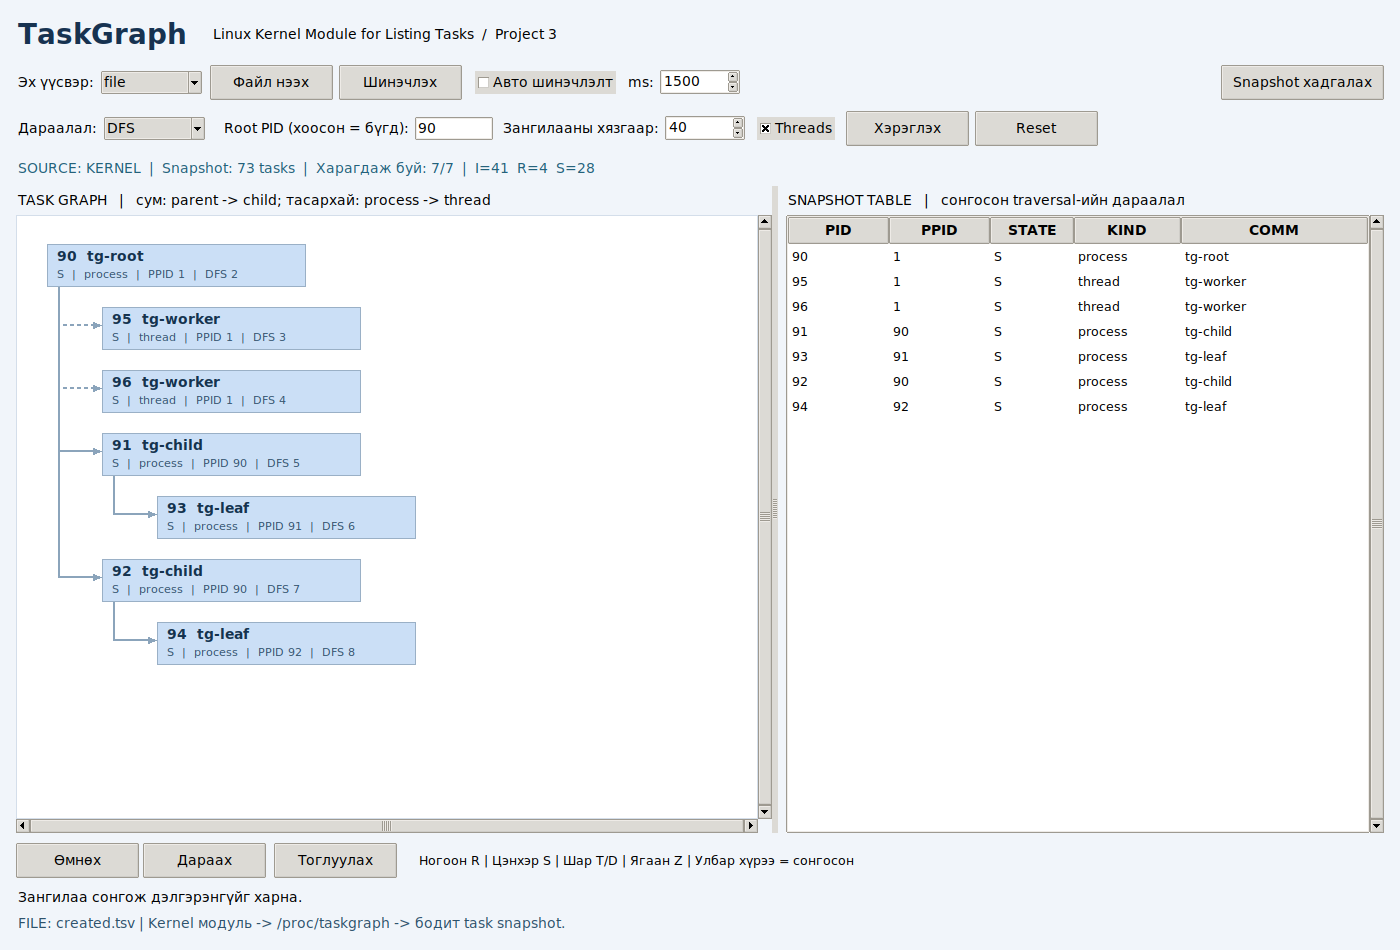
\includegraphics[width=\textwidth]{../images/kernel_created_ui.png}
\caption{Kernel-ийн created snapshot-ийг UI-д нээсэн байдал.}
\end{figure}
Root PID 90-ийн дэд модонд 7 task байна. PID 95, 96 нь thread тул тасархай сумаар холбогдсон. PID 91, 92 нь root-ийн хүүхэд; PID 93, 94 нь тэдгээрийн хүүхэд юм.
\begin{table}[H]
\centering\small
\caption{Зурагт харагдаж буй task-ууд}
\begin{tabularx}{\textwidth}{@{}P{1.8cm}P{2.8cm}P{2.8cm}Y@{}}\toprule
PID & Графын parent & Төрөл & Нэр \\\midrule
90 & 1 & Process & \code{tg-root} \\
95, 96 & 90 & Thread & \code{tg-worker} \\
91, 92 & 90 & Process & \code{tg-child} \\
93, 94 & 91, 92 & Process & \code{tg-leaf} \\\bottomrule
\end{tabularx}
\end{table}
Зургийн өгөгдлийг QEMU дахь бодит Linux kernel module-оос авч, \code{created.tsv} файлаар UI-д импортолсон. Графын холбоос, хүснэгтийн мөрүүд нэг snapshot-д тулгуурлана.

\clearpage
\subsection{Төлөвийн өөрчлөлт}
\begin{figure}[H]
\centering
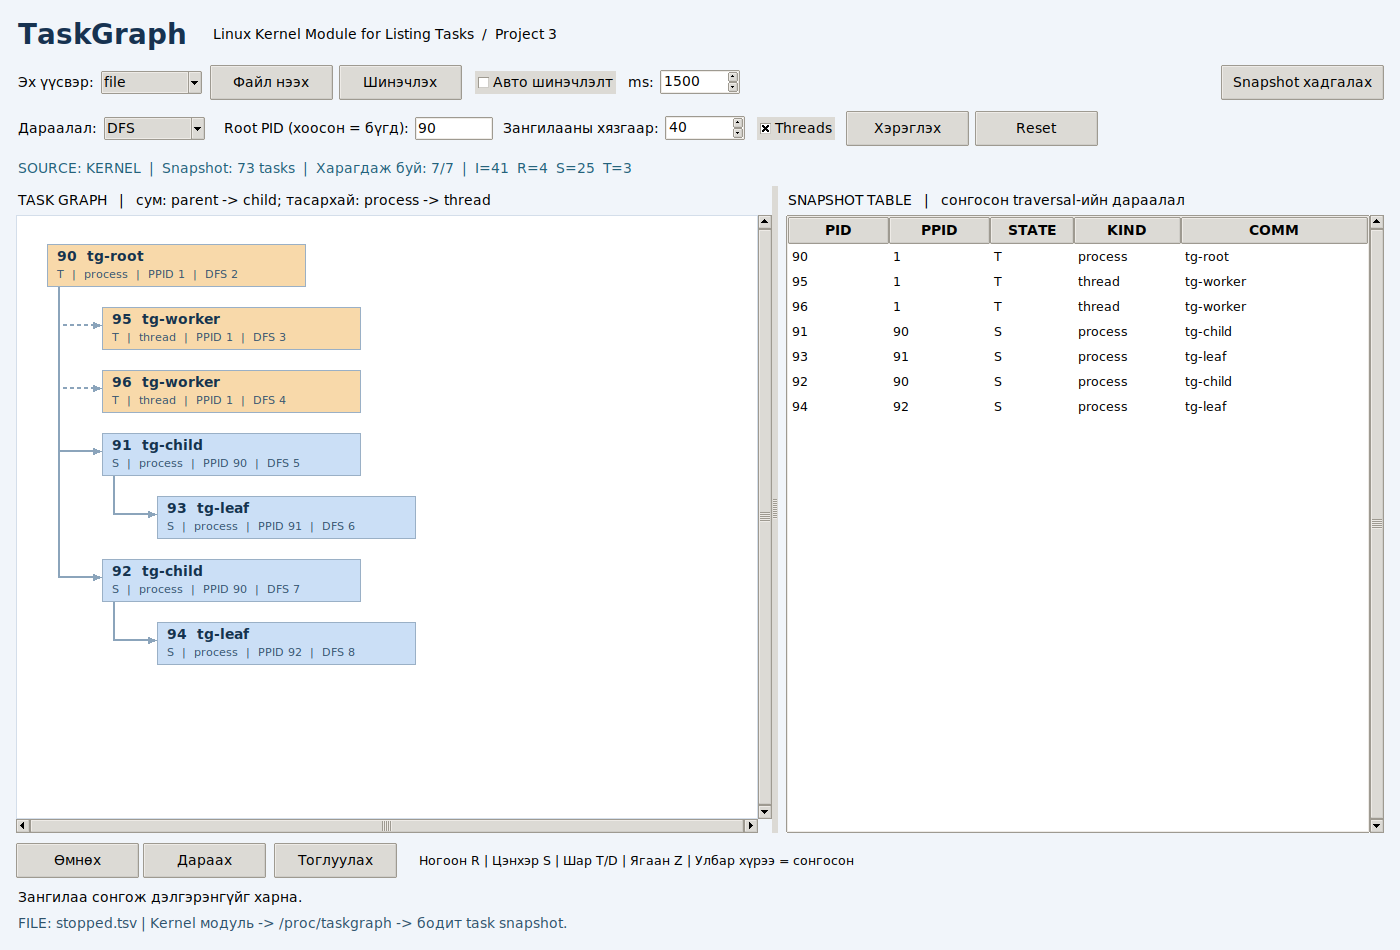
\includegraphics[width=\textwidth]{../images/kernel_stopped_ui.png}
\caption{SIGSTOP дараах snapshot: root PID 90-ийн төлөв T болсон.}
\end{figure}
SIGSTOP өгсний дараа PID 90 шар өнгөөр дүрслэгдэв. SIGCONT өгч үргэлжлүүлэн, workload-ийг дуусгахад үүсгэсэн процесс, thread-үүд цэвэрлэгдсэн. Хязгаарласан snapshot-д \code{truncated=1} тэмдэг ил тод гарсан.
\begin{table}[H]
\centering\small
\caption{Хэмжилтүүдийн харьцуулалт}
\begin{tabularx}{\textwidth}{@{}P{3cm}Y@{}}\toprule
Үе шат & Үр дүн \\\midrule
Created & Root-ийн дэд мод: 5 process + 2 thread. \\
Stopped & Root-ийн state=T. \\
After & Workload-ийн task үлдээгүй. \\
Capped & 16 мөр; snapshot дутууг тэмдэглэсэн. \\
Unloaded & Proc файл устсан. \\\bottomrule
\end{tabularx}
\end{table}

\clearpage
\section{Хэлэлцүүлэг}
Граф болон хүснэгт нь kernel-ийн PID, parent, төлөвийн мэдээлэлтэй тохирч байв. Тестээр process-thread ялгалт, DFS дараалал, STOP төлөв, буруу параметр болон модулийн цэвэрлэгээг шалгасан.
RCU нь санах ойн аюулгүй уншилтыг хангах боловч бүх системийн нэг агшны атомик зураг батлахгүй. Процесс үүсэх, дуусах үед parent олдохгүй бол root-д холбоод \code{orphan=1} гэж тэмдэглэнэ. \code{comm} нь богино task name; бүтэн командын мөр биш. Том системд \code{max\_tasks}-ийг өсгөх шаардлагатай.
Kernel ажиллагааг QEMU initramfs орчинд шалгасан. Тайлангийн UI зураг нь тэндээс авсан snapshot-ийн дүрслэл юм. Хадгалсан snapshot нь өмнөх хэмжилтийг давтан үзэхэд зориулагдсан; бодит Linux хэмжилтийг \code{--kernel} горимоор ажиллуулна.

\section{Дүгнэлт}
Процессын жагсаалтыг LINEAR болон DFS аргаар гаргах kernel module, task graph UI, snapshot хадгалах болон дахин үзэх боломжийг хэрэгжүүлэв. Нийт 35 автомат шалгалт тэнцсэн. Төслөөр Linux-ийн task бүтэц, process-thread холбоо, төлөв болон DFS-ийг бодит өгөгдөлтэй холбон судалсан.

\renewcommand{\refname}{Ашигласан материал}
\begin{thebibliography}{9}
\def\UrlFont{\ttfamily\scriptsize}
\addcontentsline{toc}{section}{Ашигласан материал}
\small
\bibitem{osc} A. Silberschatz, P. B. Galvin, G. Gagne. \textit{Operating System Concepts}. 10th ed., Wiley, 2018. Chapter 3, Programming Project 3, P-17--P-19.
\bibitem{guide} F.CSM302. \textit{Бие даалт 1-ийн удирдамж}. OS\_BD1\_Guide.pdf, 2026.
\bibitem{rcu} Linux 6.8. \textit{Using RCU to Protect Read-Mostly Linked Lists}. \url{https://docs.kernel.org/6.8/RCU/listRCU.html}
\bibitem{seq} Linux 6.8. \textit{The seq\_file Interface}. \url{https://docs.kernel.org/6.8/filesystems/seq_file.html}
\bibitem{kbuild} Linux 6.8. \textit{Building External Modules}. \url{https://docs.kernel.org/6.8/kbuild/modules.html}
\bibitem{repo} Төслийн эх код, тест, баримт бичиг.\\
\url{https://github.com/Temka0511/FCSA_302-IV-2-3-LINUX-Kernel-Module-For-Task-Information}
\end{thebibliography}
\noindent\footnotesize Код, тест, баримт бичгийг боловсруулахад ChatGPT/Codex-ийн туслалцаа ашигласан.
\end{document}
